\documentclass{article}
\usepackage{graphicx} % Required for inserting images

\usepackage[
    backend=biber,
    style=authoryear,
    sorting=ynt
]{biblatex} % Required for adding references

\usepackage[inkscapeformat=png]{svg} 
\usepackage{appendix}
\usepackage{calc}
\usepackage{float}
\usepackage{fontspec}
\usepackage{pdfpages}
\addbibresource{bibliography.bib}

\title{COMP7024 Coursework2- Developing a file encryption system for the Minix Operating System}
\author{19129163 Mohammad Ali Khan}
\date{April 2023}

\begin{document}

\maketitle

\section{Introduction}
    \paragraph{}The objective of this project is to develop a program for the Minix 3.4 Operating System (OS) that will encrypt and decrypt files on the system.
    \paragraph{}This program will be written in the C programming language, and has a GitHub repository which can be found at https://github.com/mhdl1991/19129163-COMP7024-Coursework2
    \paragraph{}This program will be developed as a \textbf{daemon}.

\section{A Brief note on Daemons}
    \paragraph{}A \textbf{Daemon} (sometimes claimed to be an acronym for\textit{Disk And Execution MONitor}) is a computer program that runs as a background process, not under direct control of a user, and supervises the system or provides functionality to other processes . Other terms for daemons include \textit{service}, \textit{ghost job}, or \textit{started task}.
    
    \paragraph{}Examples of daemons include \textbf{init}, \textbf{crond}, \textbf{httpd}, and \textbf{syncd}, all of which perform useful tasks in the operating system.

\section{Requirements}
    \paragraph{}We will need the following:
    \begin{itemize}
        \item Knowledge of the Minix OS and filesystem
        \item Knowledge of signals and signal handling
        \item libraries for performing Encrpytion and file handling (some may already be installed as part of the Minix OS)
        \item enough memory for handling the encryption and decryption
        \item Some way to store credentials (keys and initialization vectors)
        \item Some way to know which files have been encrypted and which have not
        \item permissions and policy settings to allow the daemon to alter files.
    \end{itemize}

\section{Encryption}
    \paragraph{}A common bit of advice regarding encryption is \textit{"Never roll your own cryptosystem"}- from technical and security standpoints it is better to use an existing, tried and tested cryptosystem than to develop your own- From a \textbf{technical} standpoint, it's very difficult to build your own cryptosystem and test it, and to make it \textbf{secure}, which ties into the \textbf{security} standpoint for not rolling your own cryptosystem.
    
    \paragraph{}For this software, we have the option of using \textbf{OpenSSL}, which can be installed on Minix using the \textbf{pkgin} utility.
    
    \paragraph{}As per the OpenSSL documentation, it contains RSA, SHA, DES, SSL, TLS, and AES cipher suites/families. For this program we are using 256-bit AES encryption in CBC (Cipher Block Chaining) mode, using OpenSSL's \textbf{EVP library} \parencite{openssl_evp}.

\section{Design}
    \paragraph{}the program will have two main functions, \textit{file\_encrypt} and \textit{file\_decrypt}. Both functions will take a pointer to a file, a key, and an IV (initialization vector).
    \paragraph{}the credentials (the key and IV) will be stored in an external file instead of being hard-coded into the daemon.
    \paragraph{}for handling and detecting changes to the file system, we have access to the \textbf{inotify} API \parencite{inotify_manpage}.
    

\section{Development}
    \paragraph{}The program was first built as a standalone bit of C before attempting to integrate it with the Minix operating system. This was done to make sure the file encryption and decryption functions worked properly and didn't result in bugs, memory leaks, unintended alterations to files, or other unintended consequences, and to reduce damage to the system.

    \subsection{A note on developing encryption/decryption functions}
        \paragraph{}The encryption/decryption functions were more or less adapted from sample code in the OpenSSL documentation, with added code to take the contents of a file and read them into a \textbf{unsigned char} buffer, which the OpenSSL functions for encryption/decryption accept as arguments, and then write unsigned char buffers to files after encryption/decryption.

        \begin{figure}[htbp]
            \centering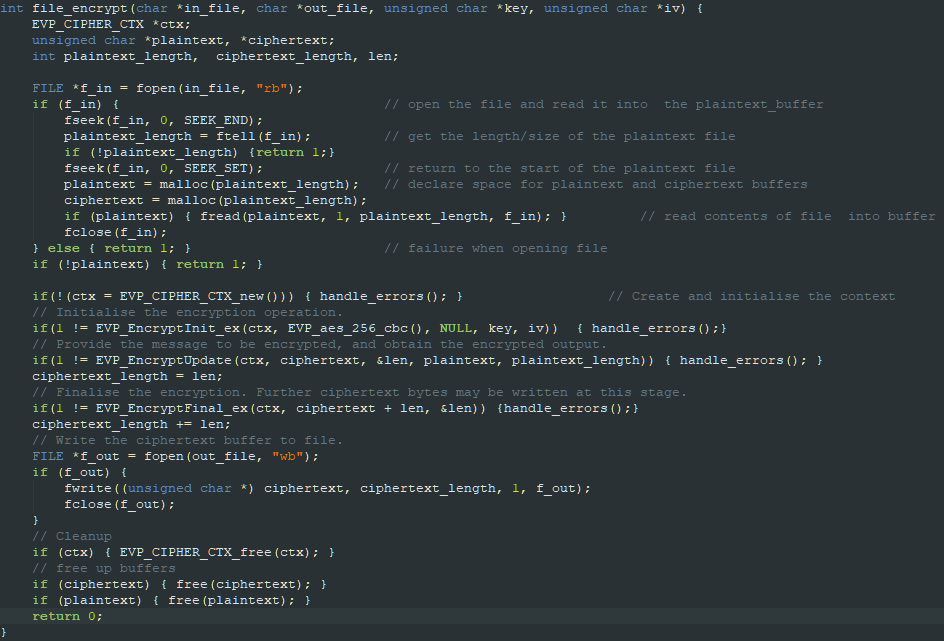
\includegraphics[width=\textwidth]{encrypt_function_screenshot_1.png}
            \caption{C function that encrypts a file using AES-256}
            \label{fig:my_label}
        \end{figure}
    \newpage
    \subsection{A note on Daemon development}
        \paragraph{}the basic principle of how a daemon operates involves the following steps:
        \begin{itemize}
            \item Fork off the parent process (usually init)
            \item Change file mode mask (umask)
            \item Opening logs for writing \textit{(optional)}
            \item Create a unique Session ID (SID)
            \item Change the current working directory
            \item Close standard file descriptors
            \item Enter actual daemon code
        \end{itemize}
        \paragraph{}It will then run until system shutdown, and handle \textbf{signals} sent by the Operating system.
        \paragraph{}Minix also provides the \textbf{daemon} command that turns other processes into daemons, automatically performing the tasks needed to set them up as such \parencite{daemon_command_minix}.

        \begin{figure}[htbp]
            \centering
            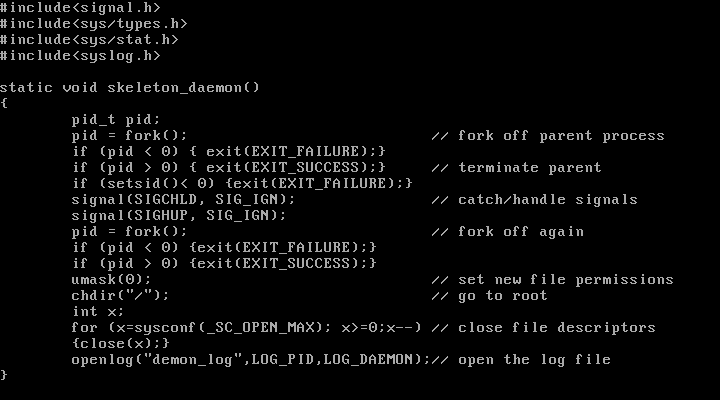
\includegraphics[width=\textwidth]{daemon_code_screenshot_1.png}
            \caption{C function that provides a "skeleton" for making a daemon}
            \label{fig:my_label}
        \end{figure}
    

\section{Testing}
    \paragraph{}The program is tested in it's standalone form first, to make sure that it is encrypting and decrypting files properly
    \paragraph{}It will be tested on a number of different file types and sizes, to see if encryption and decryption properly reverts the file back to it's former self.

\section{Conclusion}
    \paragraph{}Operating systems are remarkably complex, even Minix, an OS built as an educational tool to show how OS kernels work, has a huge degree of complexity that must be taken into account when attempting to add on or expand on it.

\printbibliography
\end{document}
